\subsection{Comparing the simulated system to the original data}

To create reusable algorithms for the simulated data, the concept of a slice is introduced. A slice is a two dimensional datastructure holding the value of the enhancement using $x$ and $y$ coordinates. These coordinates reflect the $x$ and $y$ coordinates of the overal simulation but don't have to be a plane in the $z$ plane. Instead slices can be any geometric structures representable as $z=f(x,y)$.

\begin{figure}[!h]
  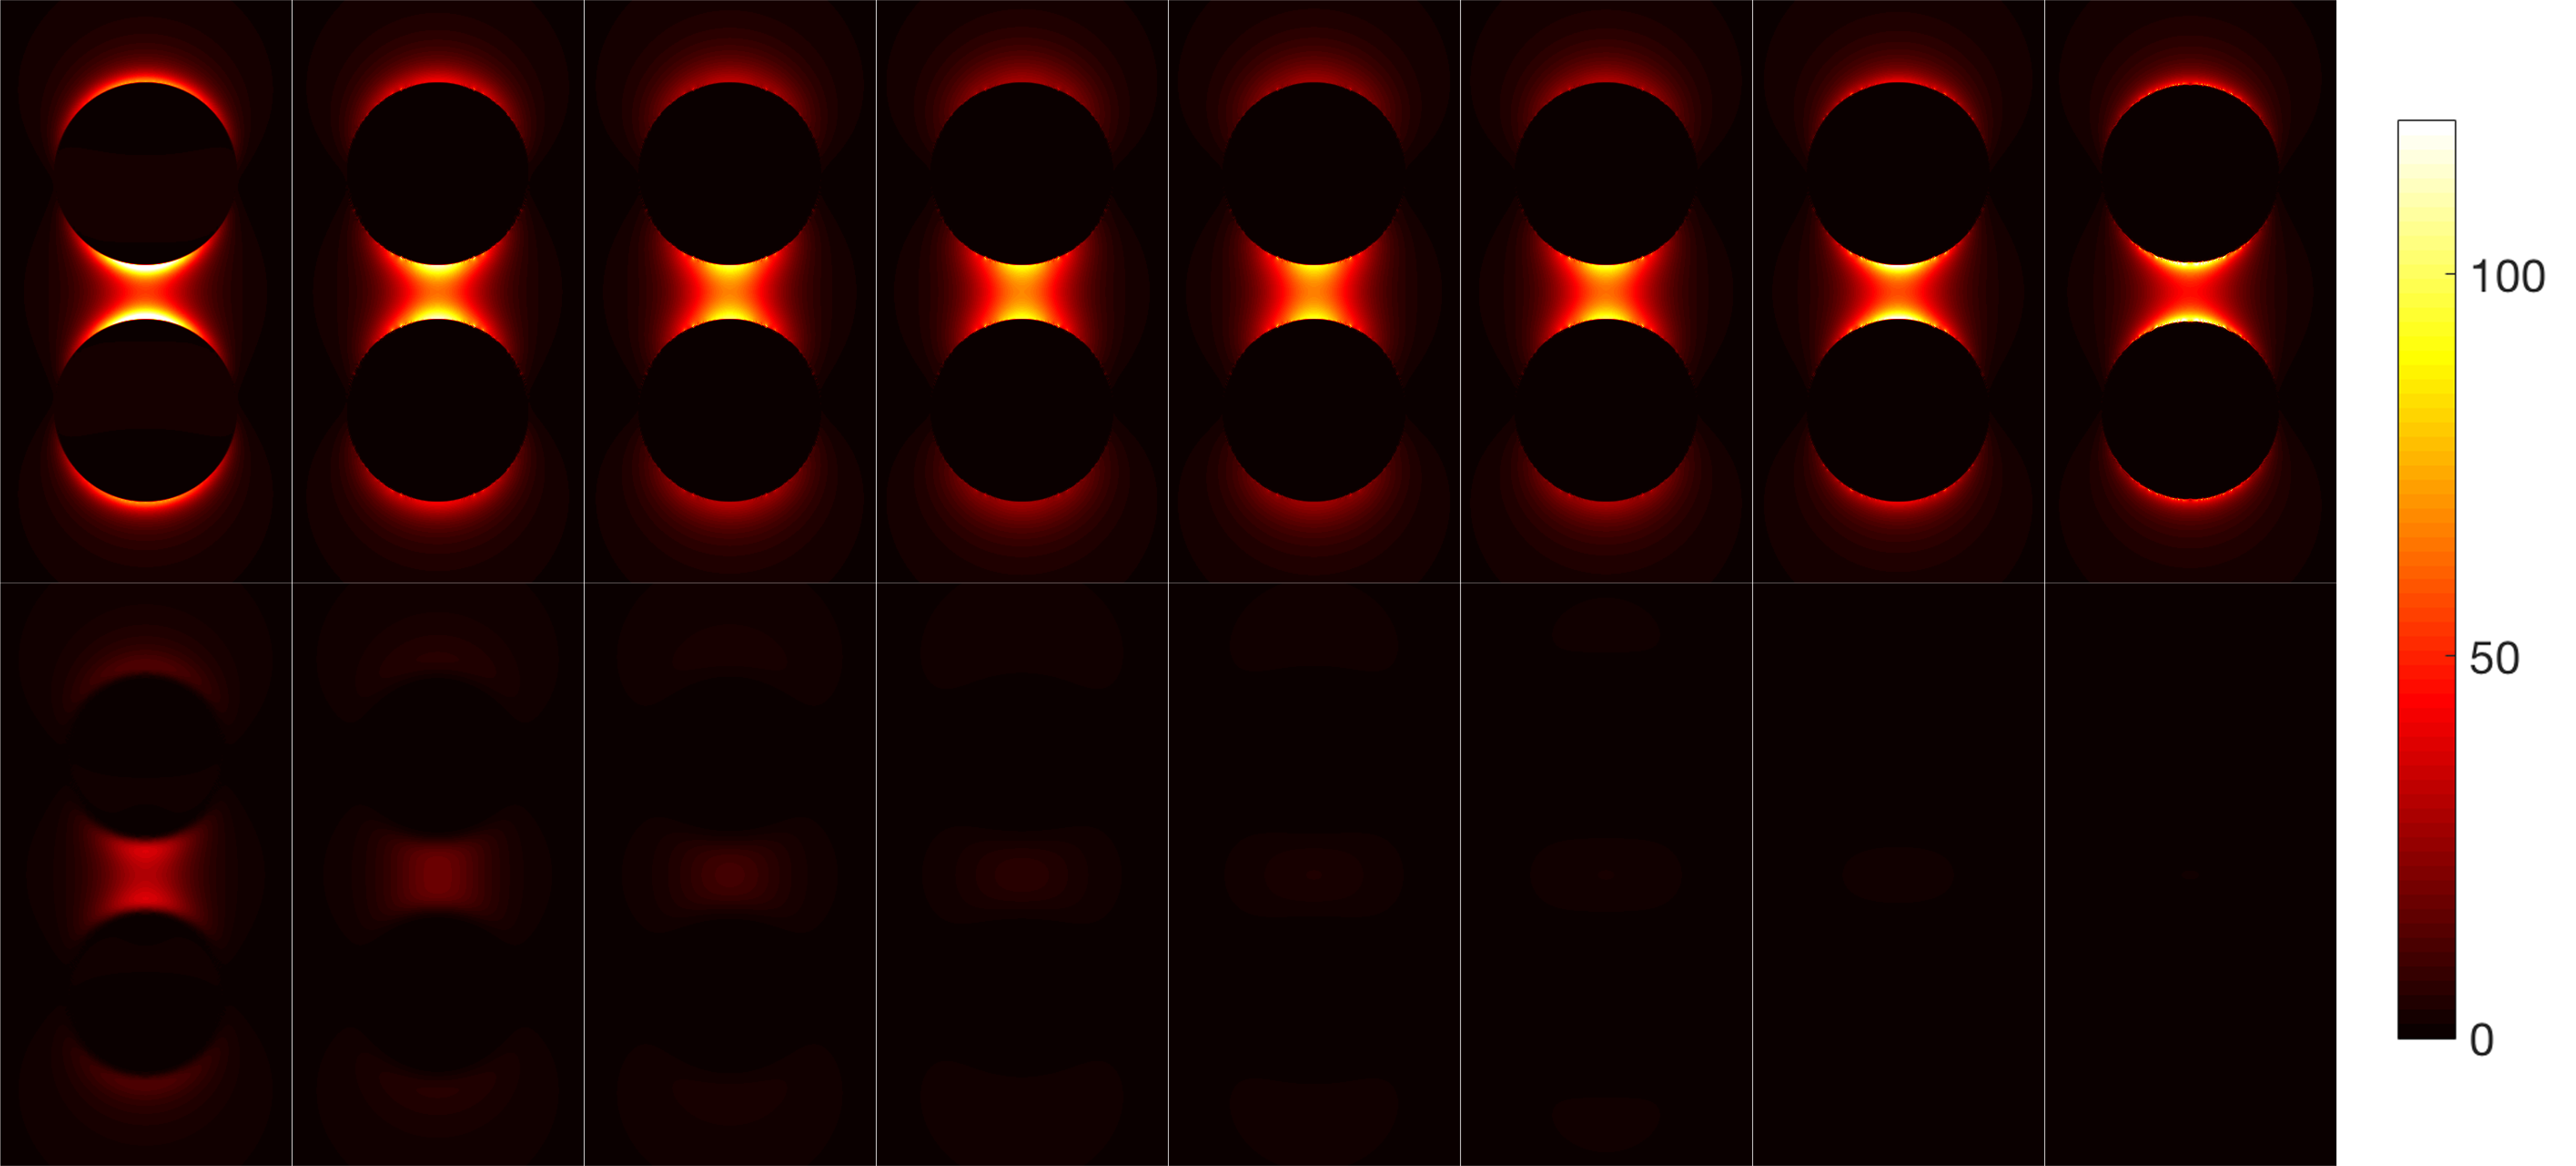
\includegraphics[width=\textwidth]{./images/simulation-slices.png}
  \label{slices}
  \caption{Slices of the simulation's result in the $x,y$-plane as near field enhancement $|E/E_0|^2$. Starting at the top left at $z=\SI{0}{nm}$ continuing in \SI{5}{nm} steps until $z=\SI{80}{nm}$.}
\end{figure}

In figure \ref{slices} there are the plotted versions of slices using equidistant planes along the $z$-axis to give an overview over the enhancement at different values of $z$. Noticeable are the fragments of spatial discretisation along the rounded gold structures.

Figure \ref{slices} shows the resonance of plasmons with light polarized in $x$-direction. The cavity between the gold nanostructures the biggest amount to the total enhancement as already shown by \cite{heeg}. Above the structure ($z>\SI{45}{nm}$) the enhancement drops off significantly.
